% % % % % % % % % % % % % % % % % %
%                                 %
%  Master Thesis                  %
%  MSc in Aerospace Engineering   %
%  Mattia Gregnanin               %
%  A.Y. 2025/2026                 %
%                                 %
% % % % % % % % % % % % % % % % % %
%                                 %
%  Chapter 1 / Section 1          %
%                                 %
% % % % % % % % % % % % % % % % % %

\section{Historical Overview}
\label{sec:history}

The history of rocket flight computer systems is closely tied to the development of rocketry and the advancement of electronic technology. One of the earliest examples of a rocket guidance system was the \emph{Mischgerät}, an electromechanical device used in the German V-2 rocket during World War II (\cref{fig:mischgerat}). It processed electrical signals from onboard spinning gyroscopes to control the rocket's flight path~\cite{cdvandt}. German engineers also pioneered radio telemetry on board rockets, transmitting sensor measurements from the vehicle to a ground station~\cite{rocketryhandbook}. Although these systems represented a significant technological achievement for their time, their complexity, weight, and specialized hardware made them unsuitable for widespread use outside military and research applications.

Following World War II, guidance and navigation systems continued to evolve alongside advances in electronics and computing. A notable milestone was the Apollo Guidance Computer (AGC), developed for NASA's Apollo missions during the 1960s. Shown in \cref{fig:agc}, it was among the first computers to make extensive use of integrated circuits, demonstrating how electronic computing could be integrated into spacecraft guidance and navigation systems~\cite{digitalapollo}. Nevertheless, the cost, complexity and specialized nature of these systems placed them well beyond the reach of amateur rocketry.

\begin{figure}[htb]
    \centering
    \begin{subfigure}{0.48\textwidth}
        \centering
        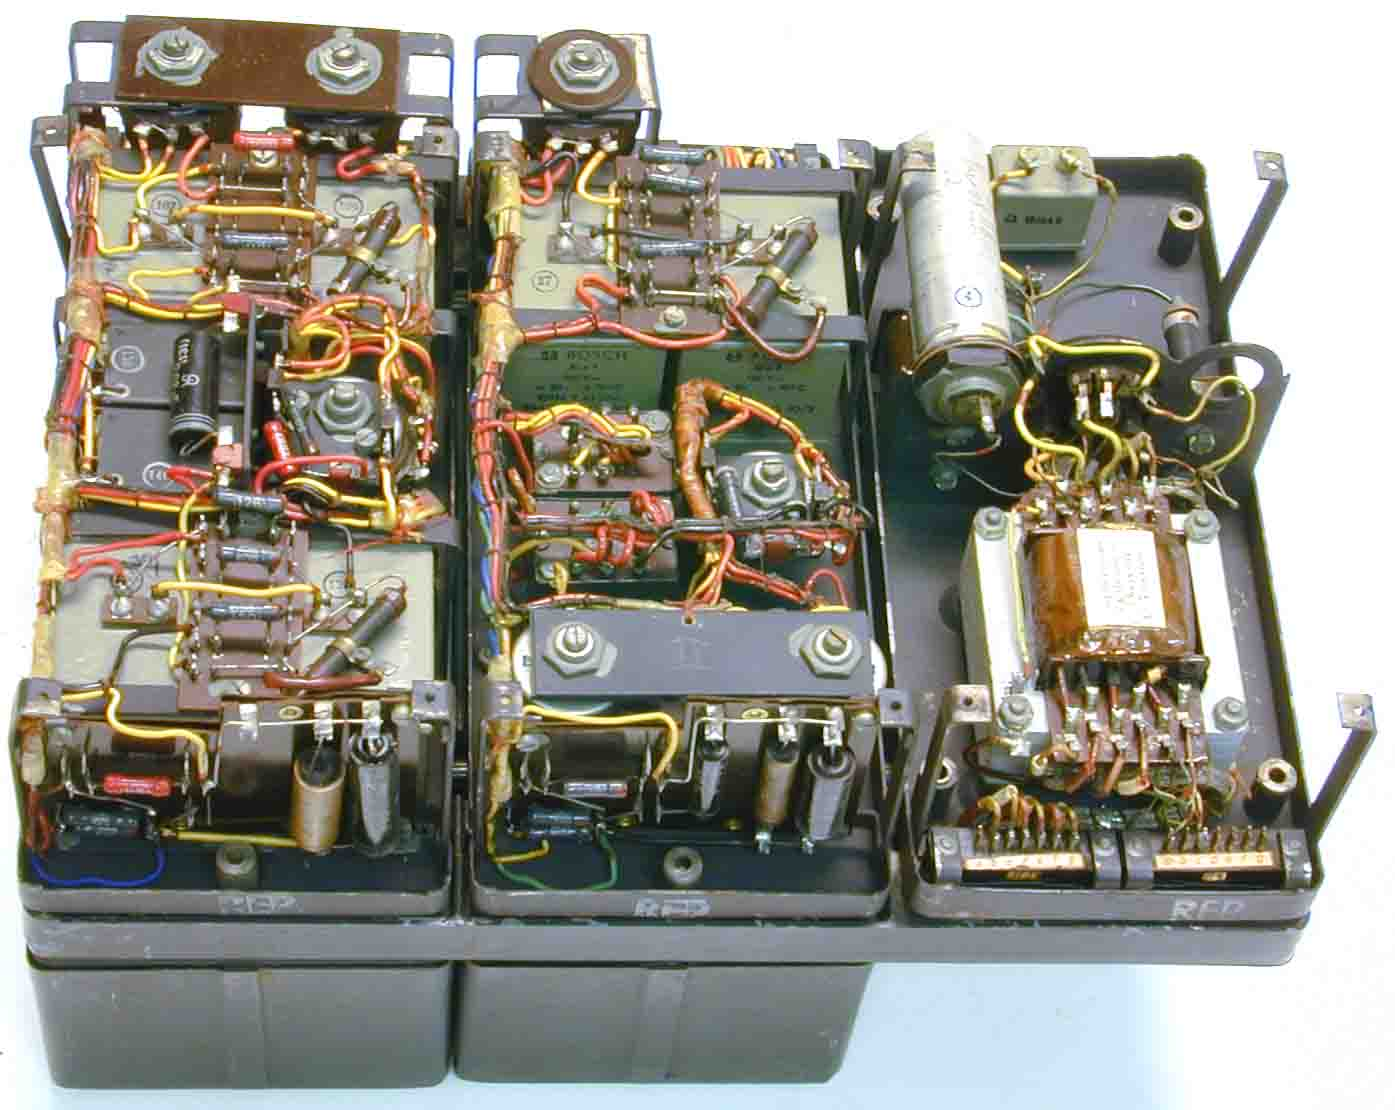
\includegraphics[width=\textwidth]{mischgerat}
        \caption{V-2 rocket control unit (Mischgerät)~\cite{cdvandt}.}
        \label{fig:mischgerat}
    \end{subfigure}
    \hfill
    \begin{subfigure}[b]{0.48\textwidth}
        \centering
        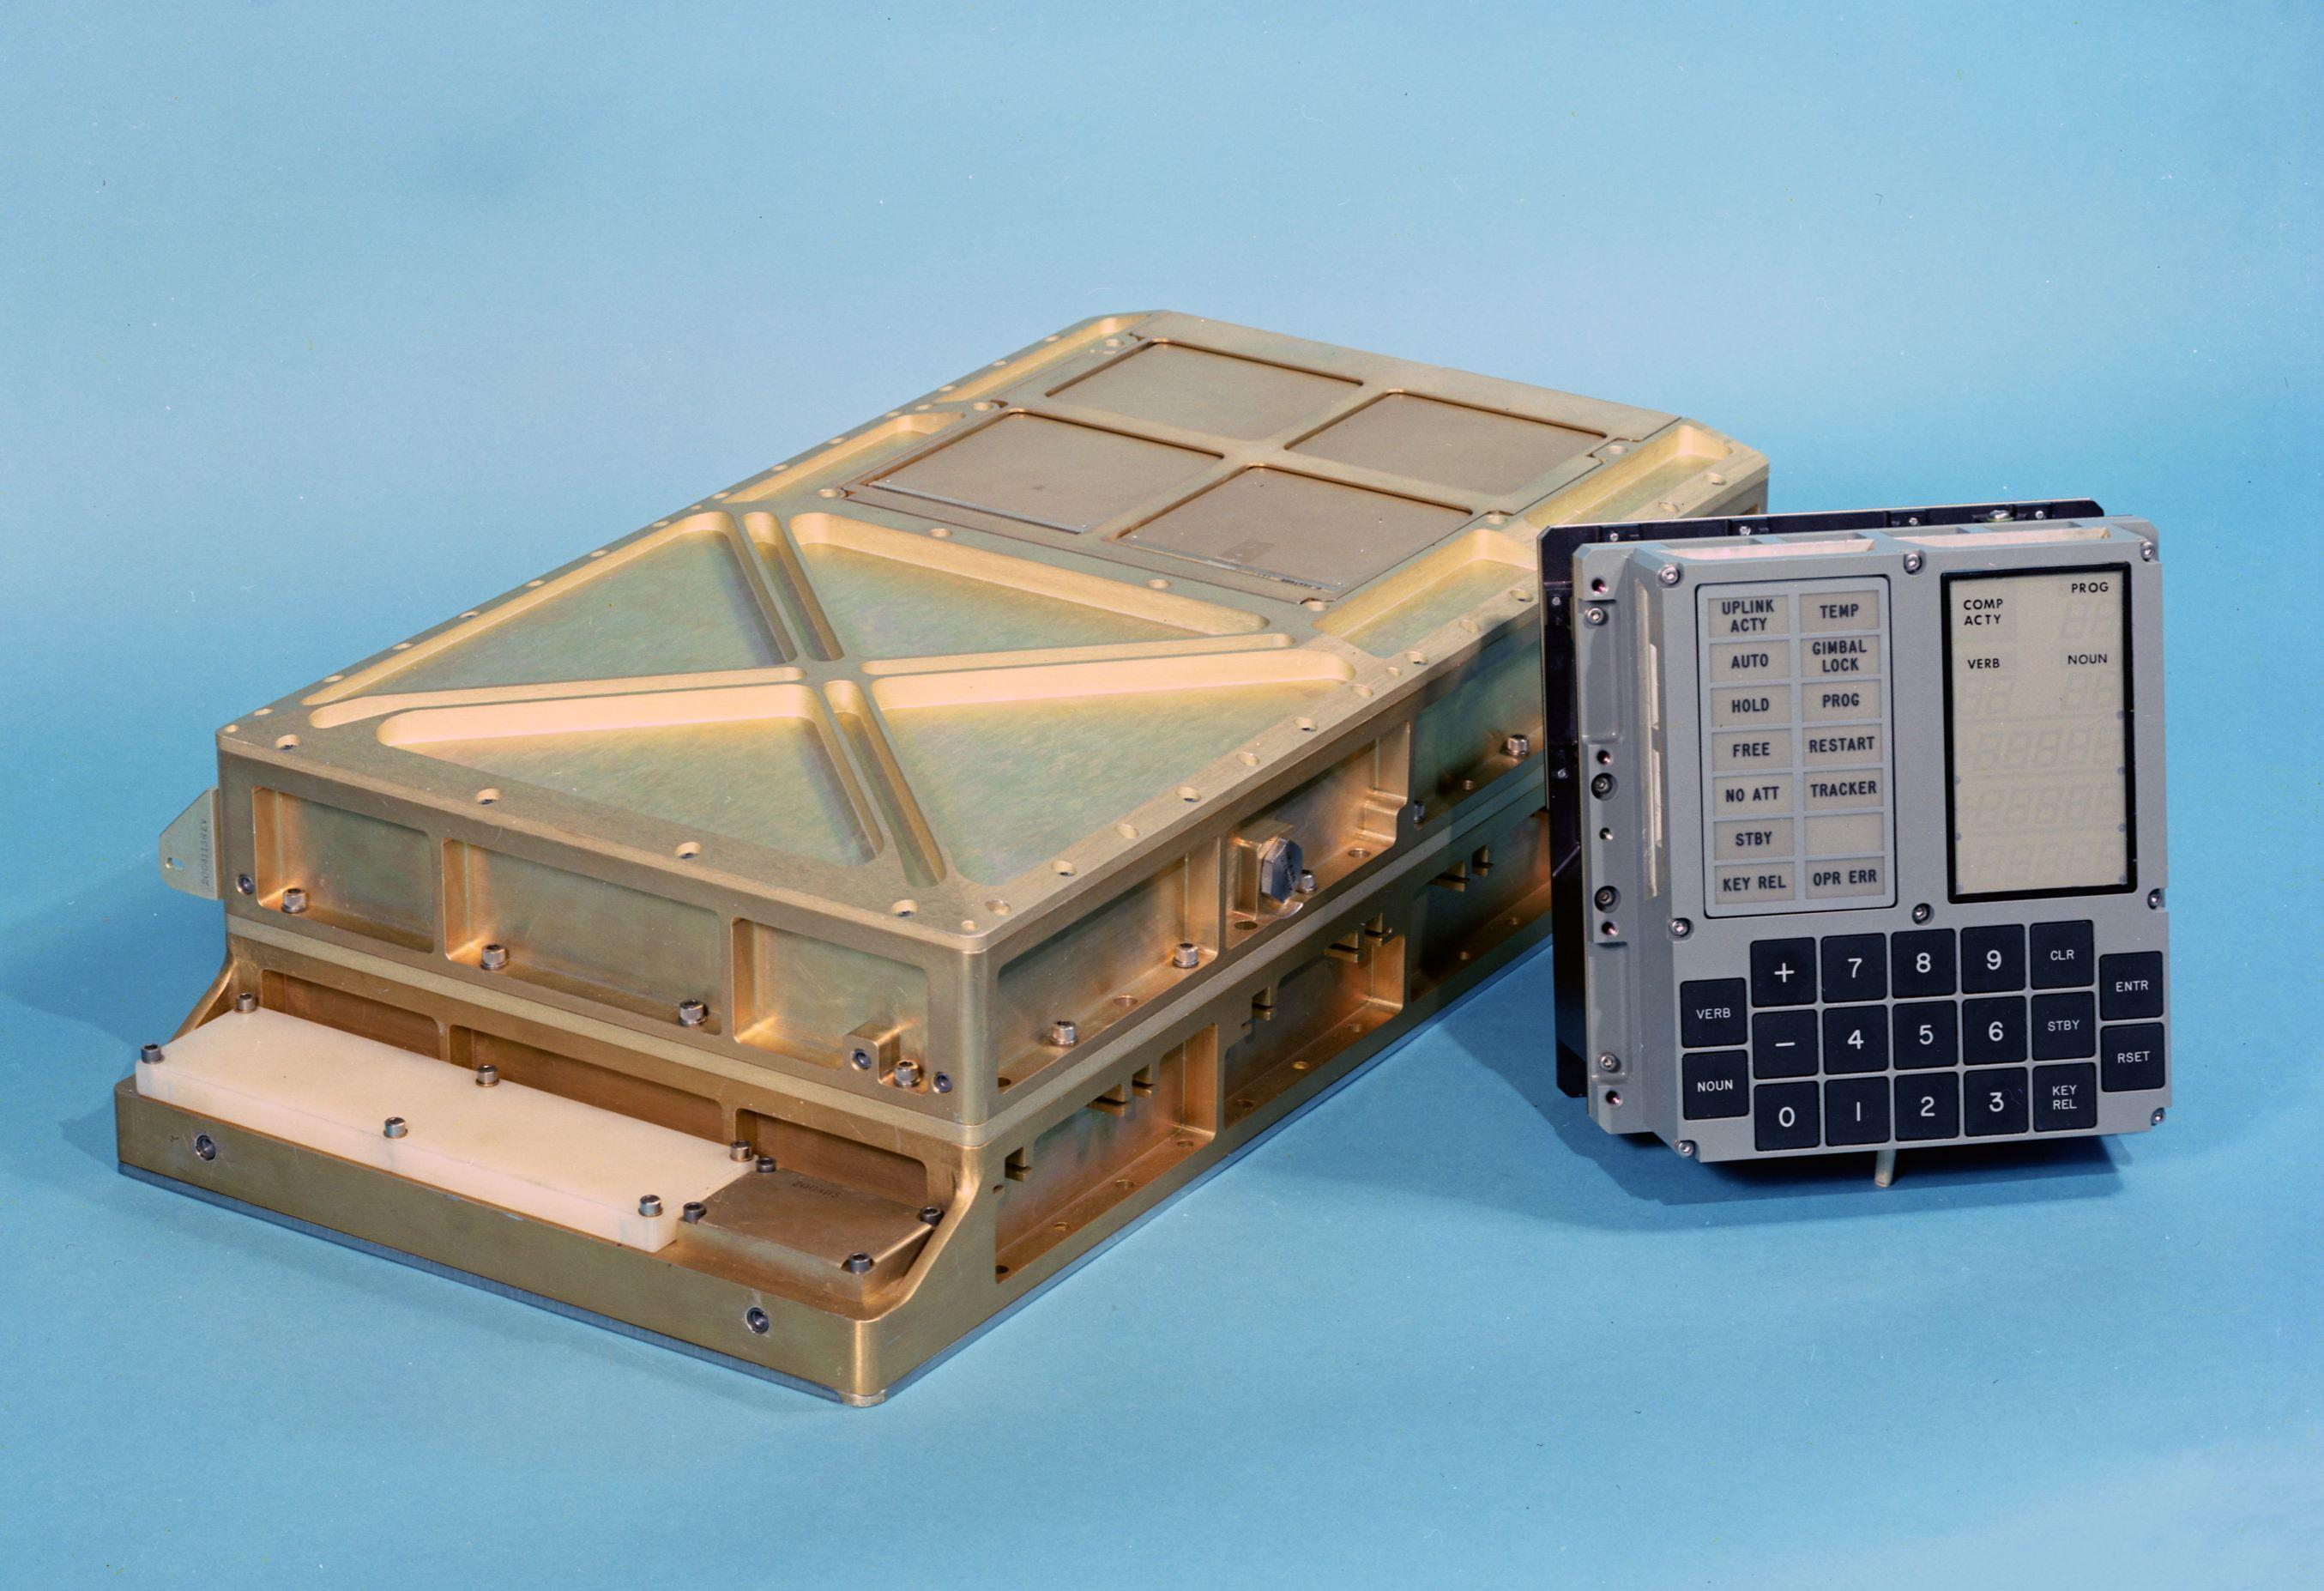
\includegraphics[width=\textwidth]{agc}
        \caption{Apollo Guidance Computer~\cite{wiki:agcview}.}
        \label{fig:agc}
    \end{subfigure}
    \caption{Historical examples of guidance systems for rockets and spacecraft.}
    \label{fig:historicalguidance}
\end{figure}

In parallel, electronics began to play an important role in amateur rocketry, initially as a means of recovering rockets after landing. The first amateur rocket transmitter, built in Colorado in 1960, emitted a signal in the \SI{27}{MHz} Citizen Band (CB) frequency band. The signal could be detected using a directional antenna to locate the rocket on the ground~\cite{rocketryhandbook}. Unlike modern telemetry systems, this initial device served only as a recovery beacon and did not transmit, at least in its early versions, flight measurements.

Beyond locating the rocket, a more fundamental requirement is its safe recovery. Model rocketry associations such as the NAR and Tripoli require that rockets be recovered in a safe manner after each flight, which also allows them to be flown again~\cite{nar:safetycode,tripoli:safetycode}.
Traditionally, recovery was triggered by the delay element built into the motor, which fires an ejection charge after burnout~\cite{rocketryhandbook}, or by simple mechanical or electronic timers. In both cases the deployment time is fixed before launch, whereas the instant of apogee depends on factors such as vehicle mass, aerodynamic drag, weather conditions and motor variability. Deployment can therefore occur too early or too late, compromising the integrity of the vehicle and the safety of the surroundings.

The subsequent development of microprocessors, microcontrollers and miniaturized sensors in the following decades progressively reduced the size, cost and power consumption of onboard electronic systems. In particular, the availability of compact inertial sensors and pressure sensors in the form of \emph{Micro Electro-Mechanical Systems} (MEMS) made it possible to integrate measurement, data processing and event detection into small, affordable devices~\cite{nato:mems}. These advances enabled amateur flight computers to measure altitude, record flight data and trigger recovery systems based on measured flight conditions rather than relying exclusively on predetermined delays.

More recently, open-source hardware and software have further lowered the barriers to developing custom flight computers. Development platforms such as Arduino and ESP32 provide accessible environments for prototyping embedded systems, while single-board computers such as Raspberry Pi can support more computationally demanding applications, including onboard video and image recording. Alongside custom-built solutions, several commercial products have been developed specifically for amateur rocketry, including the Altus Metrum TeleMetrum~\cite{altus:telemetrum}, the PerfectFlite StratoLoggerCF~\cite{perfectflite} and the Featherweight Blue Raven~\cite{featherweight:blueraven}, that will be reviewed in \cref{sec:existing}. Depending on the model, these devices combine barometric sensors, accelerometers and other instrumentation, and may provide onboard data logging, radio telemetry or recovery-event control.

\begin{figure}[htbp]
    \centering
    \begin{subfigure}[b]{0.48\textwidth}
        \centering
        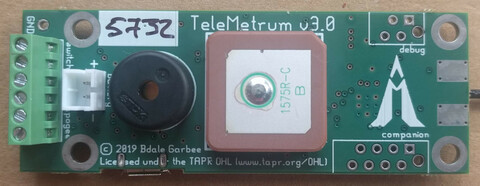
\includegraphics[width=\textwidth]{altusmetrum}
        \caption{Altus Metrum TeleMetrum~\cite{altus:telemetrum}.}
        \label{fig:altusmetrum}
    \end{subfigure}
    \hfill
    \begin{subfigure}[b]{0.48\textwidth}
        \centering
        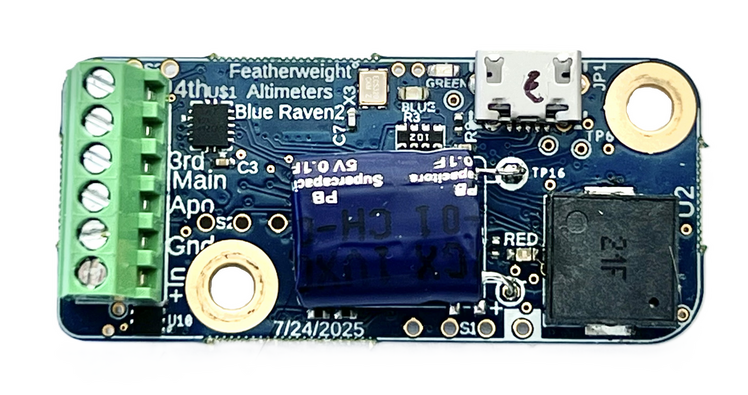
\includegraphics[width=\textwidth]{blueraven}
        \caption{Featherweight Blue Raven~\cite{featherweight:blueraven}.}
        \label{fig:blueraven}
    \end{subfigure}
    \caption{Examples of commercial flight computers for amateur rocketry.}
\end{figure}

Despite these advances, it is important to distinguish between systems primarily designed for altitude measurement and recovery, systems intended for flight-data transmission, and flight computers capable of estimating the vehicle's complete state in real time. The latter requires the integration of measurements from multiple sensors to reconstruct quantities such as attitude, position and velocity~\cite{ahrs,aiaa:rocketstateestimation}. Although these capabilities are well established in aerospace guidance and navigation systems, their implementation in compact, low-cost amateur rocket flight computers presents additional challenges in terms of computational resources, sensor integration and real-time operation.
